\documentclass[11pt]{article}
\usepackage[preprint]{acl}
\usepackage{times}
\usepackage{latexsym}
\usepackage[T1]{fontenc}
\usepackage[utf8]{inputenc}
\usepackage{microtype}
\usepackage{inconsolata}
\usepackage{graphicx}
\usepackage{amsmath}
\usepackage{amsfonts}
\usepackage{booktabs}
\usepackage{multirow}

\usepackage{booktabs}
\usepackage{tabularx}
\usepackage{array}

\title{Polygraph: Reliable ViT Error Detection from Topological Evidence-Flow}

\author{Yishai Lavi \and Noya Hochwald \and Omri Fahn \and Eran Kramf \\
  Tel Aviv University \\
  \texttt{\{yishailavi, noyahoch, omrifahn, erankramf\}@mail.tau.ac.il} \\}

\begin{document}
\maketitle

\begin{abstract}
Detecting when an image classifier fails is a fundamental challenge for the safe deployment of Vision Transformers (ViTs). Standard error detection mechanisms often depend primarily on the network's final output logits, largely ignoring the complex token-to-token routing dynamics that construct the prediction. Drawing inspiration from hallucination detection in large language models, we hypothesize that ViTs exhibit recurring topological signatures when forming incorrect predictions. In this work, we introduce Polygraph, a framework that models a frozen ViT's attention mechanism as a directed graph to capture these latent failure patterns. By deploying an edge-gated MPNN over the final transformer layer, we extract structural evidence-flow features within a single forward pass. These internal signals are then fused with the full-logit vector via a mixture gate. Evaluated on CIFAR-100-C, the graph model provides complementary predictive signal to strong output- and representation-based baselines, while topology ablations indicate a modest additional benefit from explicit graph structure. The combined Polygraph detector achieves the strongest error-detection performance among methods evaluated in the original benchmark and retains its advantage on corruption families entirely unseen during detector training. In exploratory follow-ups, graph-score fusion improves a fitted LogitDynamics adaptation, while matched set-score fusion attains almost the same point estimate; intermediate auxiliary-head projections provide a smaller improvement within the adaptation.
\end{abstract}

\section{Introduction}
Vision Transformers (ViTs) \citep{Dosovitskiy2021} construct image representations through complex, layer-wise information routing among patch tokens, yet their predictive reliability is commonly estimated from the final softmax distribution. This reliance on output scores leaves much of the internal token interaction that constructs the prediction unmodeled; predictions with similar output confidence can nevertheless arise from different internal representations and routing patterns.

To address this, we investigate error prediction through the attributed attention graph induced by a ViT. Given a frozen classifier $f$ and an input image $x$ with ground-truth label $y$, let $
\hat{y}(x)=\arg\max_c f_c(x)$, and $
e(x)=1[\hat{y}(x)\neq y]$. Our objective is to predict $e(x)$ using only signals available from a single forward pass of the frozen classifier, without external verification or additional classifier evaluations.

While recent approaches such as LogitDynamics \citep{Beigelman2026} track the layer-wise trajectory of class evidence, they do not explicitly model the token-to-token connectivity underlying these predictions. We propose Polygraph, a method that represents the final ViT block as a directed attributed graph to capture latent routing signatures. Node features are constructed from token hidden states, while edge features encode evidence-flow statistics derived from attention and class signals. An edge-gated MPNN produces a graph-based internal failure score, which is combined with a strong full-logit detector using a learned per-example mixture gate fitted on held-out validation data. The resulting detector improves over either source of evidence alone and retains its advantage on corruption families excluded from detector training. Controlled topology ablations further show that most of the predictive signal lies in the internal node and edge representations, while graph connectivity and edge alignment provide a more modest additional contribution.

We extend these findings with controlled follow-ups testing competitiveness against a fixed LogitDynamics adaptation, score complementarity, and graph specificity. These studies use distinct development protocols and complement the original non-graph controls.

\section{Related Work}

\paragraph{ViT Reliability and Attention-Based Diagnostics.}
A standard baseline for detecting classifier failures is the maximum softmax probability of the predicted class \citep{Hendrycks2017}. In Vision Transformers, attention and intermediate representations have been exploited for several purposes beyond classification: \citet{Chefer2021} for explanation, \citet{Wang2024} for token pruning, and \citet{Yang2025} for weakly supervised segmentation. \citet{Cultrera2023} use a convolutional autoencoder over ViT attention heatmaps for out-of-distribution detection, but operate on attention heatmaps rather than a token-interaction graph. The closest task-level baseline is LogitDynamics \citep{Beigelman2026}, which predicts ViT classification errors from layer-wise class-logit trajectories and stability statistics derived from intermediate representations, thus reduces each layer to a class-level evidence rather than retaining pairwise interactions among patch tokens.

\paragraph{Graph-Based Error Detection.}
Natural language processing provides the closest precedents for our work. Earlier approaches construct handcrafted structural descriptors, such as  \citet{Kushnareva2021} and \citet{Binkowski2025}. HalluZig \citep{Samaga2026} models the evolution of attention-graph topology across layers using zigzag persistence. HaluGNN \citep{Kong2026b} uses hidden states as node features and attention values as weighted edges, while CHARM \citep{Frasca2026} represents attention and activations as attributes of a token graph and applies edge-aware message passing. CausalGaze \citep{Kong2026a} further refines attention graphs using gradient-guided counterfactual sensitivity of attention edges. To our knowledge, no prior work applies graph-based message passing to per-image ViT patch-attention graphs for predicting visual classification failures. Polygraph studies this vision-specific setting.

\section{Methodology}
\begin{figure*}[t]
    \centering
    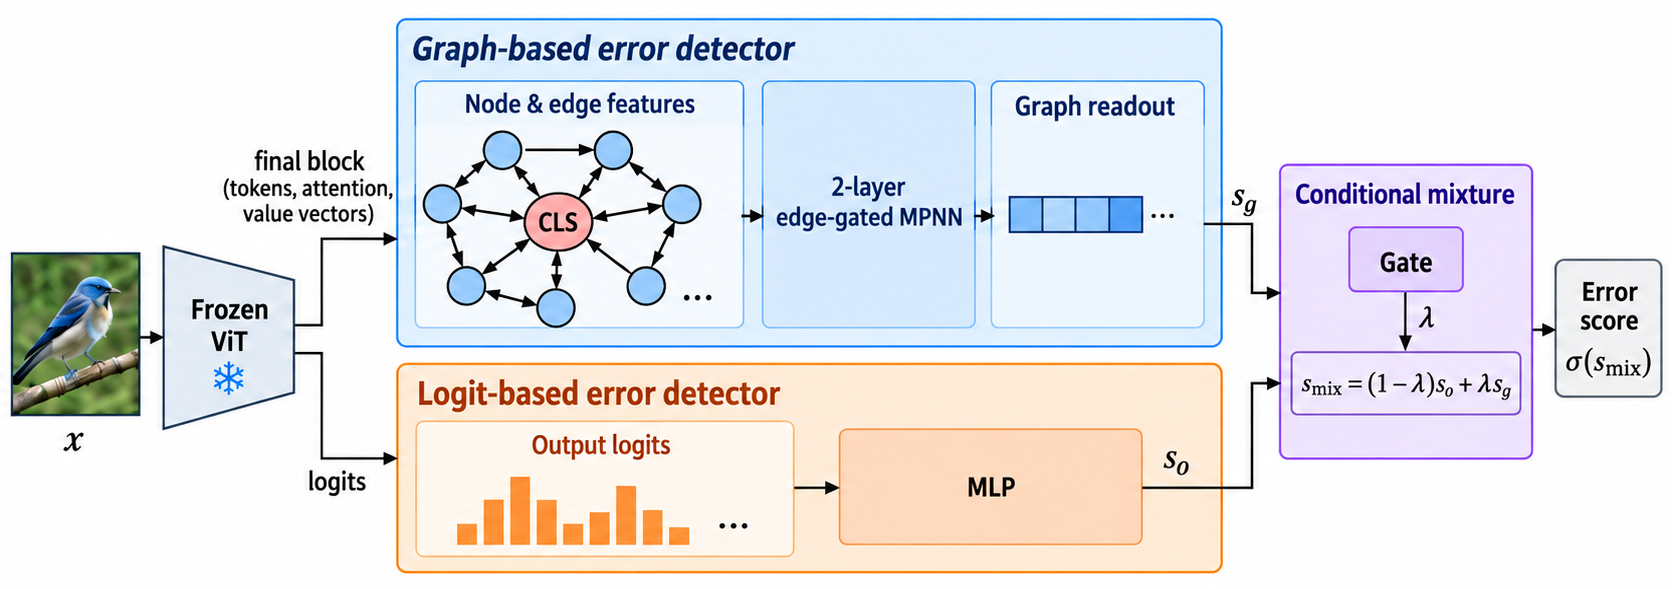
\includegraphics[width=\textwidth]{model_scheme_gnn_course.png}
    \caption{
    \textbf{Overview of Polygraph.}
    A frozen ViT provides both final-block internal representations and output logits.
    The graph branch constructs an attributed token graph from the final Transformer block,
    processes it with a two-layer edge-gated MPNN, and applies graph readout to produce an internal error score $s_g$.
    In parallel, a logit-based MLP produces an output-based error score $s_o$.
    A conditional mixture gate combines the two experts into the final failure score.
    }
    \label{fig:polygraph-overview}
\end{figure*}

Polygraph combines two complementary error detectors: one operates on the
ViT's internal attention graph, while the other operates on its output logits.
The two experts are trained independently and are subsequently combined by a
learned, image-dependent mixture.

\subsection{Final-Block Attention Graph}

For an image $x$, let the frozen ViT produce class logits
$\boldsymbol{\ell}=f(x)\in\mathbb{R}^{C}$. We construct a graph from its final
Transformer block, containing $N$ tokens and $H$ attention heads. Let
$\mathcal{V}=\{0,\ldots,N-1\}$ denote the token set, with token $0$ representing
CLS. For head $h$, $A_{ij}^{(h)}$ denotes the attention assigned by query token
$i$ to key token $j$. We orient the corresponding edge as $j\rightarrow i$.

We retain an edge whenever it receives sufficiently high attention in at least
one head:
\begin{equation}
\mathcal{E}
=
\left\{
(j,i):
j\neq i,\;
\max_h A_{ij}^{(h)}>\tau
\right\}
\label{eq:edge-set}
\end{equation}

Self-edges are excluded from $\mathcal{E}$, but their diagonal attention values
are retained as node attributes.

For each token $i$, the node feature $\mathbf{x}_i$ concatenates its normalized
patch coordinates, a CLS indicator, the diagonal attention values
$\{A_{ii}^{(h)}\}_{h=1}^{H}$, and its final-block hidden representation. 

\subsection{Evidence-Flow Edge Features}

Raw attention describes how strongly token $i$ reads from token $j$, but not
the content or direction of the information being transmitted. We therefore
augment every retained edge with two additional per-head features.

Let $\mathbf{v}_j^{(h)}$ denote the value vector of source token $j$ in head
$h$, and let $\mathbf{W}_O^{(h)}$ denote the corresponding part of the
multi-head output projection. Their product
\begin{equation}
\mathbf{u}_j^{(h)}
=
\mathbf{W}_O^{(h)}\mathbf{v}_j^{(h)}
\label{eq:transformed-value}
\end{equation}
represents the contribution of that value after projection back into the
Transformer hidden space.

To measure how strongly this contribution supports the model's current
decision, let $\hat c$ and $\tilde c$ be the classes with the highest and
second-highest output logits. If $\mathbf{w}_c$ denotes the frozen classifier
weight vector for class $c$, we define the normalized predicted-versus-runner-up
direction
\begin{equation}
\mathbf{d}
=
\frac{
\mathbf{w}_{\hat c}-\mathbf{w}_{\tilde c}
}{
\left\|
\mathbf{w}_{\hat c}-\mathbf{w}_{\tilde c}
\right\|_2
}
\label{eq:class-direction}
\end{equation}

For each retained edge $j\rightarrow i$ and head $h$, we then compute an
attention-weighted magnitude feature and a signed class-direction feature:
\begin{equation}
\begin{aligned}
m_{ji}^{(h)}
&=
\log\!\left(
1+
A_{ij}^{(h)}
\left\|
\mathbf{u}_j^{(h)}
\right\|_2
\right)
\\
c_{ji}^{(h)}
&=
\operatorname{asinh}\!\left(
A_{ij}^{(h)}
\mathbf{d}^{\top}\mathbf{u}_j^{(h)}
\right)
\end{aligned}
\label{eq:evidence-features}
\end{equation}

The first captures the magnitude of the transmitted contribution, whereas the
second measures whether it aligns with the classifier's current
predicted-versus-runner-up direction. The complete edge attribute $\mathbf{e}_{ji}$ concatenates over all heads the described features. No ground-truth label is used in their construction.

\subsection{Edge-Gated Graph Detector}

We process the attributed graph using a two-layer edge-gated MPNN. Node and edge attributes are first mapped by learned projections to a
shared latent representation.

At message-passing layer $r$, each edge $j\rightarrow i$ produces both a
candidate message and an element-wise gate:
\begin{equation}
\begin{aligned}
\boldsymbol{\mu}_{ji}^{(r)}
&=
M_r\!\left(
[
\mathbf{h}_j^{(r-1)}
\,\|\,
\widetilde{\mathbf{e}}_{ji}
]
\right)
\\
\boldsymbol{\gamma}_{ji}^{(r)}
&=
\sigma\!\left(
G_r\!\left(
[
\mathbf{h}_j^{(r-1)}
\,\|\,
\mathbf{h}_i^{(r-1)}
\,\|\,
\widetilde{\mathbf{e}}_{ji}
]
\right)
\right)
\end{aligned}
\label{eq:message-gate}
\end{equation}
where $\mathbf{h}_i^{(r)}$ is the latent state of node $i$ after layer $r$,
$\widetilde{\mathbf{e}}_{ji}$ is the projected edge attribute and $M_r$ and $G_r$ are learned affine maps.

For the incoming neighborhood
$\mathcal{N}_i^-=\{j:(j,i)\in\mathcal{E}\}$, the gated messages are aggregated
as
\begin{equation}
\overline{\boldsymbol{\mu}}_i^{(r)}
=
\frac{
\sum_{j\in\mathcal{N}_i^-}
\boldsymbol{\gamma}_{ji}^{(r)}
\odot
\boldsymbol{\mu}_{ji}^{(r)}
}{
\sum_{j\in\mathcal{N}_i^-}
\boldsymbol{\gamma}_{ji}^{(r)}
}
\label{eq:gated-aggregation}
\end{equation}
where $\odot$ denotes element-wise multiplication.

Each node is updated from its previous state, the aggregated
message, and its log-in-degree $\log(1+|\mathcal{N}^{-}_i|)$,
using an MLP with dropout, a residual connection, LayerNorm,
and ReLU.

After message passing, we combine the final CLS-node state with a learned
weighted pooling of all token states. Let $\psi$ be a learned scalar node
scorer and $\rho$ the final graph decoder. The graph error logit is
\begin{equation}
\begin{aligned}
\beta_i
&=
\frac{
\exp\!\left(\psi(\mathbf{h}_i)\right)
}{
\sum_{j\in\mathcal{V}}
\exp\!\left(\psi(\mathbf{h}_j)\right)
}
\\
s_g(x)
&=
\rho\!\left(
[
\mathbf{h}_{0}
\,\|\,
\sum_{i\in\mathcal{V}}
\beta_i\mathbf{h}_i
]
\right)
\end{aligned}
\label{eq:graph-readout}
\end{equation}

Thus, the detector retains direct access to the CLS token while also learning
which patch-token representations are informative for failure prediction.

\subsection{Output Expert and Conditional Fusion}

The second expert operates directly on the complete output-logit vector and
produces an error logit $s_o(x)$. The output MLP receives the full logit vector, standardized
per class using detector-training statistics. The graph and output experts are trained
independently using class-weighted binary cross-entropy against
\begin{equation}
Y_{\mathrm{err}}(x)
=
1
\left[
\hat c\neq y
\right]
\label{eq:error-target}
\end{equation}
where $y$ is the ground-truth class. 

Once trained, both experts are frozen. Their scores are independently
calibrated on held-out meta-validation data, producing calibrated logits
$z_o(x)$ and $z_g(x)$. A small gate receives the standardized pair of expert
scores and predicts an example-specific graph weight $\lambda(x)\in[0,1]$:
\begin{equation}
z_{\mathrm{mix}}(x)
=
\left(
1-\lambda(x)
\right)z_o(x)
+
\lambda(x)z_g(x)
\label{eq:conditional-mixture}
\end{equation}

Equation~(9) is applied separately in each of five grouped
meta-validation folds. Each fold fits its score standardizer,
scalar logistic calibrators, and gate on four folds, using the
remaining fold for gate early stopping. At test time, we average
the five mixture logits; both frozen experts are shared across
folds.

The gate therefore learns when the internal graph signal provides useful
information beyond the output-logit expert. To avoid leakage, calibration and
gate fitting are performed only on a disjoint meta-validation split using
grouped cross-validation by original image.

\paragraph{Implementation details.}
In our experiments, the ViT has $N=197$ tokens, $H=12$ heads,
$D=768$, and per-head dimension $64$. We use $\tau=0.02$, resulting in
approximately $7{,}600$ directed edges per image. Node features contain 16
base attributes plus the 768-dimensional hidden state, and edge attributes
contain 36 values (12 attention, 12 magnitude, and 12 class-direction
features). The graph detector uses latent width 64, two message-passing layers,
and dropout $0.15$. The output expert has dimensions
$100\!\rightarrow\!64\!\rightarrow\!32\!\rightarrow\!1$, and the mixture gate
uses $2\!\rightarrow\!16\!\rightarrow\!1$. We use five grouped folds for
mixture fitting.

\section{Experimental Setup}

This section describes the original Polygraph experiments; the follow-ups use the distinct protocols in Section~\ref{sec:controlled-followups}.

\subsection{Datasets and Splits}
We evaluate on CIFAR-100 and CIFAR-100-C using a frozen ViT-B/16
pretrained on ImageNet-21k and fine-tuned on CIFAR-100. We construct an error-balanced benchmark by sampling equal
numbers of correct and incorrect predictions within each
source--severity stratum. All versions of the same original
image remain in one train/validation/test partition. We consider
the main benchmark and a weather-family holdout in which selected
corruption families are excluded from detector training and used to
evaluate distribution-shift generalization. Model selection uses only
the corresponding validation split, and results for these original experiments are on
held-out test data.

\subsection{Training and Baselines}
We select models by validation AUROC with early stopping and repeat
all learned detectors over three random seeds. We compare against
maximum softmax probability (MSP) and a strict output-only MLP trained
on the complete classifier-logit vector. 

% Vertically centered cell: mean above, standard deviation below.
\newcommand{\pgscore}[2]{%
  \begingroup
  \renewcommand{\arraystretch}{0.85}%
  \begin{tabular}[c]{@{}c@{}}%
    #1\\
    {\scriptsize\(\pm\,#2\)}%
  \end{tabular}%
  \endgroup
}

\section{Results}

\subsection{Main Error Detection}
Table~\ref{tab:results_main} compares detectors on the main
CIFAR-100/CIFAR-100-C test split. Polygraph improves mean AUROC over
the strict full-logit MLP, while also improving AUPRC and
AURC. The standalone graph expert provides a smaller mean AUROC
gain. Throughout this section, \emph{graph expert} denotes
the selected two-layer edge-gated MPNN, and \emph{Polygraph} denotes
its conditional fusion with the output MLP.

\begin{table}[!htbp]
  \centering
  \small
  \setlength{\tabcolsep}{3pt}
  \renewcommand{\arraystretch}{1.08}
  \begin{tabularx}{\columnwidth}{@{}>{\raggedright\arraybackslash}Xccc@{}}
    \toprule
    Method & AUROC $\uparrow$ & AUPRC $\uparrow$ & AURC $\downarrow$ \\
    \midrule
    MSP          & 0.8651          & 0.8345          & 0.2218 \\
    Output MLP   & 0.8794          & 0.8583          & 0.2158 \\
    Graph expert & 0.8883          & 0.8682          & 0.2105 \\
    Polygraph    & \textbf{0.8939} & \textbf{0.8748} & \textbf{0.2071} \\
    \bottomrule
  \end{tabularx}
  \caption{Main-test performance, averaged over three seeds for
  learned detectors. MSP is deterministic. Bold marks the best
  result in each column.}
  \label{tab:results_main}
\end{table}

Using 2,000 paired bootstrap repetitions grouped by original image,
the 95\% confidence interval for the Polygraph--output AUROC
difference lies above zero in all three seeds. The standalone graph
improvement is less certain, although at an equal flagging budget of 50\% of test examples per
detector, the graph expert identifies 37.4\% of the true errors
missed by the output MLP, averaged across seeds. These distinct error sets
support using the graph score as complementary evidence.

\paragraph{Corruption severity.}
Table~\ref{tab:results_severity} reports the main-test breakdown
by corruption severity. Polygraph has the highest mean AUROC at
each severity from 1 to 5. The graph expert alone
also exceeds the output MLP at every reported severity.

\begin{table}[!htbp]
  \centering
  \small
  \setlength{\tabcolsep}{3pt}
  \renewcommand{\arraystretch}{1.16}
  \begin{tabularx}{\columnwidth}{@{}c*{4}{>{\centering\arraybackslash}X}@{}}
    \toprule
    Severity & MSP & \shortstack{Output\\MLP}
      & \shortstack{Graph\\expert} & Polygraph \\
    \midrule
    1 & 0.8928 & 0.8967 & 0.8978 & \textbf{0.9065} \\
    2 & 0.8904 & 0.8977 & 0.9047 & \textbf{0.9115} \\
    3 & 0.8727 & 0.8804 & 0.8905 & \textbf{0.8957} \\
    4 & 0.8537 & 0.8743 & 0.8857 & \textbf{0.8907} \\
    5 & 0.8184 & 0.8537 & 0.8673 & \textbf{0.8707} \\
    \bottomrule
  \end{tabularx}
  \caption{Main-test AUROC by corruption severity, pooling
  corruption types within each severity. Learned-detector values
  are three-seed means.}
  \label{tab:results_severity}
\end{table}

\subsection{Held-Out Corruption Generalization}
Under the weather-family holdout, Polygraph improves over the
output MLP on both the complete test set and the subset containing
only unseen weather and extra corruptions
(Table~\ref{tab:results_weather}). On the unseen subset, Polygraph also
exceeds MSP, whereas the standalone graph expert and the
output MLP do not exceed MSP. Thus, conditional fusion retains
its benefit for corruption types excluded from detector training.

\begin{table}[!htbp]
  \centering
  \small
  \setlength{\tabcolsep}{4pt}
  \renewcommand{\arraystretch}{1.08}
  \begin{tabularx}{\columnwidth}{@{}>{\raggedright\arraybackslash}Xcc@{}}
    \toprule
    Method
      & \shortstack{Full test\\AUROC $\uparrow$}
      & \shortstack{Unseen only\\AUROC $\uparrow$} \\
    \midrule
    MSP          & 0.8625          & 0.8844 \\
    Output MLP   & 0.8690          & 0.8816 \\
    Graph expert & 0.8764          & 0.8840 \\
    Polygraph    & \textbf{0.8820} & \textbf{0.8912} \\
    \bottomrule
  \end{tabularx}
  \caption{Weather-holdout AUROC, averaged over three seeds for
  learned detectors. Full test includes seen and unseen corruption
  families; Unseen only contains the held-out weather and extra
  corruptions.}
  \label{tab:results_weather}
\end{table}

\subsection{Representation and Topology Ablations}
\paragraph{Feature ablations.}
The TransformerConv feature study (Table~\ref{tab:ablations})
separates the effects of node and edge attributes. With base node
features, adding class direction raises AUROC substantially, whereas message magnitude alone adds little. Combining
magnitude with direction does not improve over direction alone.
With full hidden-node inputs held fixed, replacing raw-attention
edges with full evidence-flow features additionally increases AUROC.

\begin{table}[!htbp]
  \centering
  \small
  \setlength{\tabcolsep}{3pt}
  \renewcommand{\arraystretch}{1.12}
  \begin{tabularx}{\columnwidth}{@{}l>{\raggedright\arraybackslash}Xr@{}}
    \toprule
    Nodes & Edge features & AUROC $\uparrow$ \\
    \midrule
    Base    & Attention             & 0.8348 \\
    Base    & Attention + magnitude & 0.8369 \\
    Base    & Attention + direction & 0.8660 \\
    Base    & Full evidence flow    & 0.8655 \\
    \addlinespace[3pt]
    Compact & Full evidence flow    & 0.8773 \\
    \addlinespace[3pt]
    Hidden  & Attention             & 0.8754 \\
    Hidden  & Full evidence flow    & \textbf{0.8863} \\
    \bottomrule
  \end{tabularx}
  \caption{Feature ablations with TransformerConv (seed 7,
  original validation split). Compact nodes add class-conditioned
  summaries; hidden nodes add full token states. Full evidence
  flow includes attention, magnitude, and class direction.}
  \label{tab:ablations}
\end{table}

\paragraph{Non-graph controls.}
Table~\ref{tab:topology} compares models under disjoint validation data for expert selection and
fusion. All models receive the same hidden-node inputs. The
node/edge-set control pools node and edge features separately,
without retaining their incidence; the endpoint-set control
retains local source--target--edge records but performs no message passing. Both nearly match TransformerConv. The edge-gated MPNN has the highest mean AUROC.

\begin{table}[!htbp]
  \centering
  \small
  \setlength{\tabcolsep}{4pt}
  \renewcommand{\arraystretch}{1.08}
  \begin{tabularx}{\columnwidth}{@{}>{\raggedright\arraybackslash}Xc@{}}
    \toprule
    Internal detector & AUROC $\uparrow$ \\
    \midrule
    TransformerConv                 & 0.8845 \\
    Token set, no edges$^{\dagger}$ & 0.8838 \\
    Node/edge sets, no incidence    & 0.8834 \\
    Endpoint sets, no message passing & 0.8813 \\
    Edge-gated MPNN                 & \textbf{0.8883} \\
    \bottomrule
  \end{tabularx}
  \caption{Main-test topology controls under the strict validation
  protocol. All models use hidden-node inputs. Values are three-seed
  means except $^{\dagger}$, which uses seed 7 only.}
  \label{tab:topology}
\end{table}

\subsection{Architecture and Depth}
Validation screening favored the edge-gated MPNN over the tested  TransformerConv, GINE, and GATv2 variants. Their validation AUROCs were 0.8849, 0.8763, 0.8753, and 0.8759,
respectively. The selected edge-gated model has 132k parameters,
compared with 191k for the TransformerConv model.
For the edge-gated architecture, two message-passing layers
achieved 0.8849 validation AUROC, compared with 0.8792 for one
layer and 0.8789 for four.

Extending the representation to the final four ViT blocks did
not improve the tested models. 4-layer variants achieved test AUROCs of 0.8771 and 0.8820,
respectively, versus 0.8894 for the final-block edge-gated expert
at the same seed. These results support the selected configuration within the evaluated
architectures.

\section{Controlled Follow-up Studies}
\label{sec:controlled-followups}

We retain the frozen ViT-B and group each source photograph's nine views: clean, plus Gaussian noise, motion blur, fog, and JPEG at severities 3/5. Unlike the original benchmark, these cohorts are not error-balanced. Subsequent comparisons reuse examined development data; they are exploratory, not independent confirmation.

\paragraph{When does graph processing help?}
A separate five-seed study found a rich36 graph--set AUROC difference of $+0.006233$ (95\% interval $[0.002618,0.009836]$), versus $-0.003686$ ($[-0.008349,0.001045]$) with attention-only inputs. Rich36 combines per-head attention, projected-message magnitude, and signed predicted-versus-runner-up class support. A later raw12 study instead trains separate detectors on attention layers 3/6/9/12, all sharing H12 token states. Both arms receive identical 784-dimensional node values and 12 attention edge values; retained edges zero-fill head values at or below $0.02$, unlike the original all-head representation. The graph arm uses two width-64 edge-gated blocks with CLS/gated pooling; the width-84 set arm pools node/edge values separately, discarding endpoint associations. Parameters are closely matched (130,434/131,126), but endpoint treatment and pooling differ.

The later detectors complete 20 epochs on 1,600 training photographs, selecting by AUROC on 400 others. Their within-seed mean sigmoid scores define $G$ and $S$; prior graph fits are reused. Their AUROC gap is $+0.000336$ (six-contrast-adjusted $99\frac{1}{6}\%$ interval $[-0.002800,0.003409]$); $G$ reaches $0.888895$, versus $0.883127$ for the fitted single-final-layer control. Separate detectors followed by score combination differ from the joint multi-block representations above. No matched four-model final-layer ensemble isolates layer diversity. Cohorts, features, budgets and constructions differ across studies, precluding a controlled replication comparison or attribution of the changed gap to richness or ensembling.

\paragraph{LD comparison and readout decomposition.}
Our fixed LogitDynamics (LD) adaptation~\citep{Beigelman2026} trains linear class heads on all 12 CLS layers, then a standardized linear error readout. This is a ViT-Base adaptation, not a reproduction of the published ViT-Large study or the earlier local CLS-sequence GRU baseline. We allocate 1,200/800/400/800 source photographs to head fitting/readout fitting/checkpoint selection/development evaluation. Heads complete 16 epochs; readouts complete 100 with validation average-precision (AP) selection. Seeds are 7/17/27. The shared evaluation has 7,200 views and 2,271 errors; families differ in inputs, supervision, parameters and budgets.

\begin{table}[!htbp]
  \centering
  \small
  \begin{tabularx}{\columnwidth}{@{}>{\raggedright\arraybackslash}Xr@{}}
    \toprule
    Model & AUROC \\
    \midrule
    \multicolumn{2}{@{}l}{\textit{Preserved comparator families}} \\
    Graph-score ensemble $G$ & 0.8889 \\
    Set-score ensemble $S$ & 0.8886 \\
    Full-logit MLP $O$ & 0.8757 \\
    \midrule
    \multicolumn{2}{@{}l}{\textit{Nested LD readouts}} \\
    $A$: six original-classifier features & 0.8636 \\
    $B$: $A$ + layer-12 auxiliary block & 0.8948 \\
    $C$: all 12 auxiliary blocks + original & 0.8990 \\
    $D$: $C$ + seven dynamics features & 0.8981 \\
    \bottomrule
  \end{tabularx}
  \caption{Mean seed-specific AUROC on the same 800 development photographs. Comparator families are not matched to the nested LD ablation. Only readouts $A/B/C$ are newly fitted; auxiliary heads and full $D$ are preserved.}
  \label{tab:followup-ld}
\end{table}

Each numeric block contains the original classifier's predicted-class logit and five largest competing logits. $A$ is therefore not full-logit MLP $O$. Only $A/B/C$ are newly fitted, reusing heads and full adaptation $D$ (Table~\ref{tab:followup-ld}). The earlier $G-D$ contrast is $-0.009171$ (ordinary 95\% interval $[-0.015874,-0.002361]$), favoring LD over this preserved ensemble, not comparing LD to original rich conditional Polygraph. $B-A=+0.031233$ is the largest observed ablation increment. Intermediate projections add $C-B=+0.004135$ (adjusted $[0.000428,0.007911]$), with a lower bound close to zero. $D-C=-0.000900$ (secondary 95\% $[-0.001750,-0.000048]$): the dynamics block, including class-identity information, did not improve this fitted recipe. These increments neither isolate supervision causally nor explain the entire LD--GNN gap.

\paragraph{Do weaker scores still complement LD?}
We split the examined 800 photographs into 400 for combiner fitting and 400 for assessment, preserving all views. For each seed, identical standardized L2 logistic regressions combine $D+G$, $D+S$, or $D+D'$. Scaling/fitting use only the fitting subset. $D$ is the preserved pre-sigmoid error logit, left uncalibrated; $G/S$ are mean probabilities. This is not the original calibrated nonlinear five-fold mixture gate. Cyclic $D'$ pairs (7--17, 17--27, 27--7) overlap and are not independent repetitions.

\begin{table}[!htbp]
  \centering
  \small
  \begin{tabularx}{\columnwidth}{@{}>{\raggedright\arraybackslash}Xr@{}}
    \toprule
    Model & AUROC \\
    \midrule
    LD $D$ & 0.9001 \\
    Graph ensemble $G$ & 0.8956 \\
    Set ensemble $S$ & 0.8950 \\
    $D+G$ & 0.9073 \\
    $D+S$ & 0.9073 \\
    $D+D'$ & 0.9021 \\
    \bottomrule
  \end{tabularx}
  \caption{Original fitted models' mean seed-specific AUROC on the separate 400-photo fusion assessment (3,600 views). Values are not directly comparable with Table~\ref{tab:followup-ld} or the original benchmark.}
  \label{tab:followup-fusion}
\end{table}

Graph fusion improves LD by $+0.007203$ (adjusted $[0.003415,0.011330]$), despite weaker standalone $G$. However, $DG-DS=+0.000043$ (adjusted $[-0.001311,0.001508]$) shows no demonstrated graph-specific benefit (Table~\ref{tab:followup-fusion}). In the secondary comparison, graph--LD fusion also outperformed the tested two-seed LD combination: $DG-DD'=+0.005213$ (95\% $[0.001942,0.008673]$). This control is not compute-matched and establishes neither superiority over generic ensembling generally nor a graph-specific benefit.

\paragraph{Uncertainty and scope.}
AUROC treats error as positive and averages seed-specific metrics, not merged predictions. Resampling pairs source photographs, retaining nine views and shared draws across methods/seeds. The two new studies use 2,000 draws: fusion independently resamples fitting/assessment photographs and refits combiners; decomposition resamples evaluation only. Intervals condition on fixed base detectors/partition or all fitted readouts, respectively. Bonferroni adjustment across $DG-D$, $DG-DS$, and $C-B$ yields individual $98\frac{1}{3}\%$ percentile intervals; secondary 95\% intervals are descriptive. Neither correction nor additional seeds remove development-data exposure. Nonsignificance is not equivalence, and complementarity does not establish topology's necessity.

\section{Conclusion}

We introduced Polygraph, a graph-based framework for error detection in Vision Transformers that models token interactions as an evidence-flow graph and combines this internal signal with the classifier output through a conditional gate. The resulting model improves over the strongest output-only baseline and remains competitive under distribution shift. Exploratory follow-ups show graph/set scores complementing LD without a demonstrated graph-specific fusion advantage. Together, these results suggest that the tested internal-feature scores provide complementary information to output confidence and can improve failure prediction in vision transformers.

\bibliography{custom}
\end{document}
